\documentclass{article}
%Para imagenes
\usepackage{graphicx}
\usepackage{float}
\usepackage[margin=2cm]{geometry} % Ajusta todos los márgenes a 2 centímetros



\begin{document}
	\begin{titlepage}
		\centering
		{\bfseries\LARGE Universidad de Granada\par}
		\vspace{1cm}
		{\scshape\Large Facultad de Ingeniería Informática \par}
		\vspace{3cm}
		{\scshape\Huge Practica 1: Patrones de diseño \par}
		\vspace{3cm}
		{\itshape\Large DS: Grupo 1.7\par}
		\vfill
		{\Large Autores : \par}
			{\Large  Emanuel Giraldo Herrera\par}
			{\Large  Thomas Lang \par}
			{\Large  Timur Sorokin \par}
			{\Large  Alejando Iborra Morán \par}
		\vfill
		{\Large (2023-2024) \par}
	\end{titlepage}
	
	\section{Ejercicio 1 (Java)}
	\subsection{Análisis}
	Se trata de realizar una simulación de carreras de bicicletas con las siguientes características:
	\begin{itemize}
		\item \textbf{Bicicleta}\\
		Cada bicicleta tiene un identificador. Existen dos tipos de bicicletas:
		\begin{itemize}
			\item Carretera
			\item Montaña
		\end{itemize}
		

			\item \textbf{Carrera}\\
			No se conoce el número de bicicletas antes de que empiece la carrera. Además, para cada tipo de bicicleta existe su tipo de carrera con las siguientes peculiaridades:
			\begin{itemize}
				\item Carretera\\
				Antes de finalizar 10\% bicicletas abandonan la carrera
				\item Montaña\\
				Antes de finalizar 20\% bicicletas abandonan la carrera.
				\item Hebras\\
				Se utilizarán las hebras para la simulación simultanea de varias carreras
		\end{itemize}

Finalmente, los objetivos que se buscan son aplicar dos patrones de diseño: Factoría Abstracta y Factoría método.

	\end{itemize}

\subsection{UML}
Antes de realizar la implementación primero hemos de plantear el diagrama UML que relacione las entidades del problema y refleje sus interacciones.
\begin{figure}[h]
	\centering
	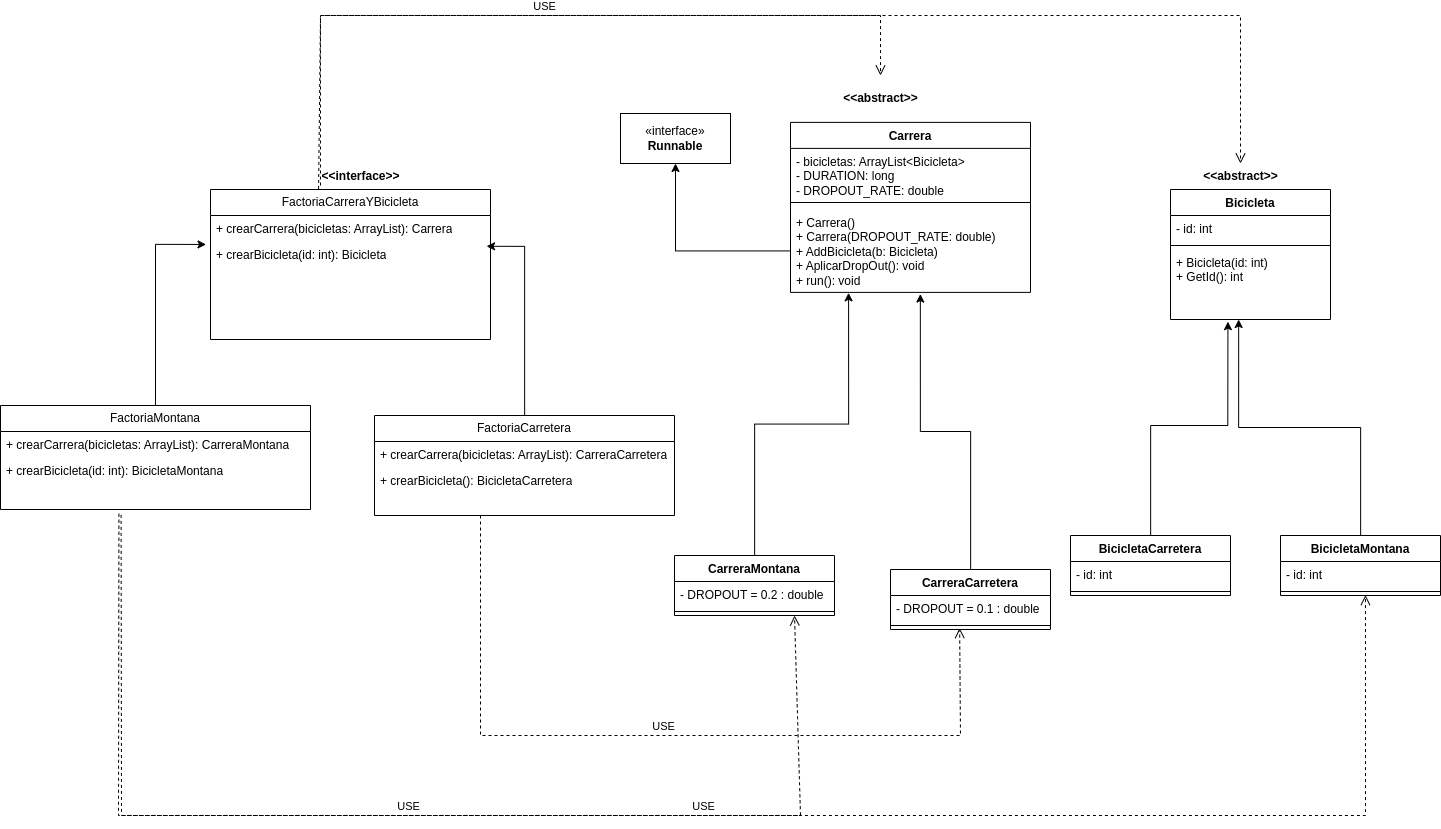
\includegraphics[width=1\textwidth]{DS_ej1.drawio.png}
	\caption{Factoría Abstracta}
	\label{fig:factoria_abstracta}
\end{figure}

\newpage
\begin{figure}[h]
	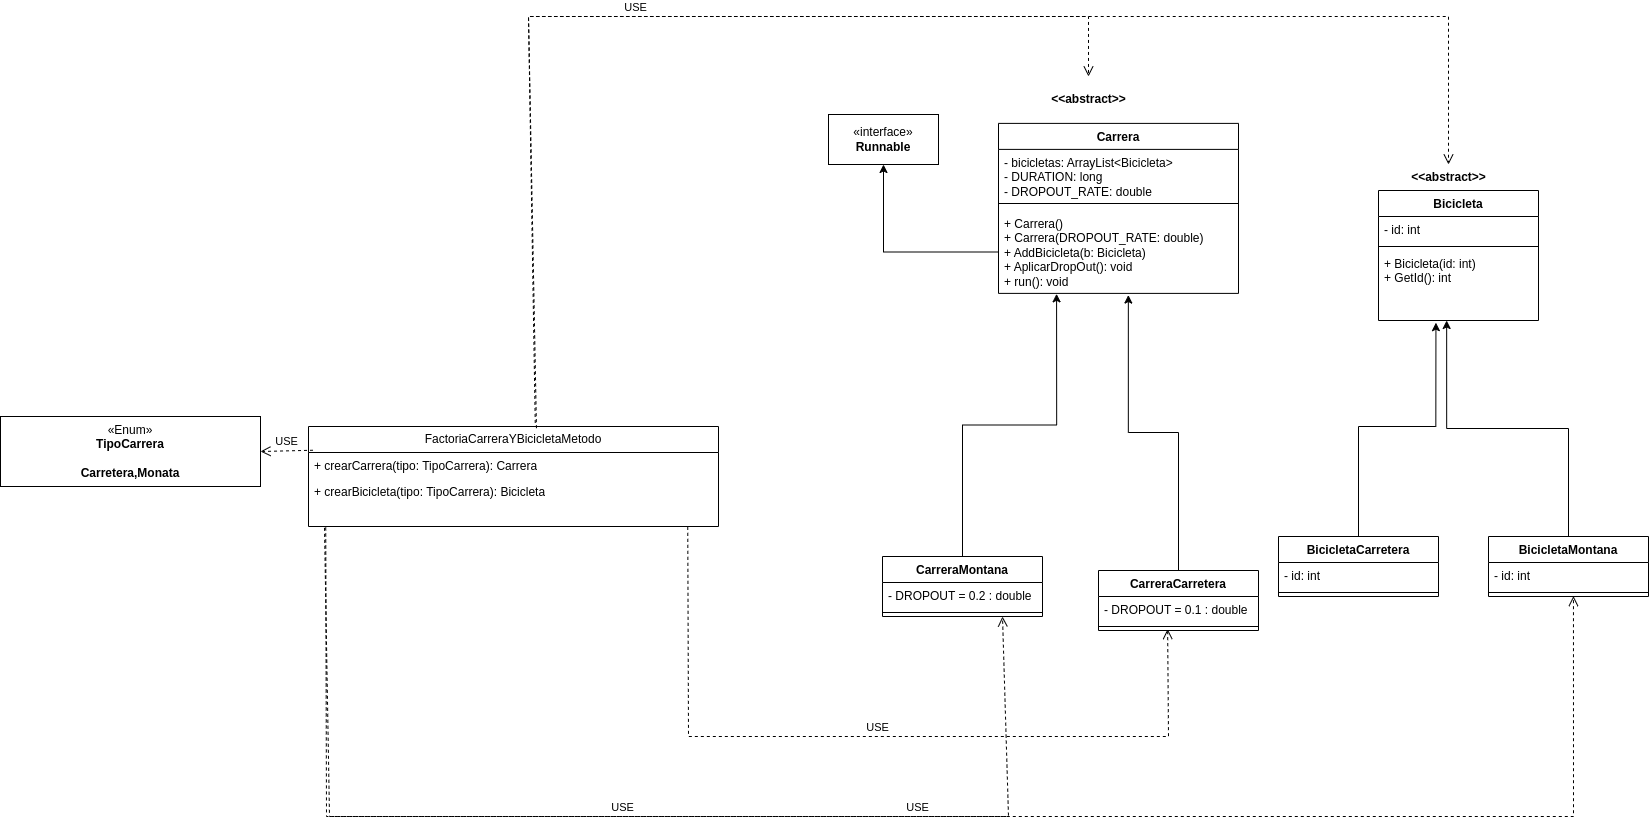
\includegraphics[width=1\textwidth]{factoria_metodo.png}
	\caption{Factoría Método}
	\label{fig:factoria_metodo}
\end{figure}

\subsection{Factoría Abstracta}
Se trata de un patrón creacional que define una interfaz para crear objetos relacionados sin especificar las clases concretas de esos objetos. Así conseguimos que el código cliente pueda instanciar los objetos sin conocer sus tipos concretos. Esto nos permite desacoplar las implementaciones concretas del código cliente. \\

En nuestro problema tenemos dos entidades básicas que son \textit{Bicicleta} y \textit{Carrera}. Hemos visto durante el análisis que existe una relación entre estas  dos clases, es decir, en una \textit{Carrera} compiten las \textit{Bicicletas}. También vimos que ambas entidades pueden ser de dos tipos: \textit{carretera} y \textit{montaña}. Cada uno de ellos con sus características \textit{concretas}. 
Entonces, tenemos que en una \textit{Carrera de montaña} participan \textit{Bicicletas de montaña}. Y en una \textit{Carrera de carretera} participan \textit{bicicletas de carretera}.  Por tanto distinguimos los siguientes elementos:
\begin{itemize}
	
	\item  \textbf{\textit{Bicicleta}}\\ Es una entidad que representa una bicicleta abstracta y actúa como una base para los distintos tipos de bicicletas que pueden existir.
	\begin{itemize}
		\item \textbf{BicicletaCarretera}\\\textit{Es una} bicicleta concreta con características añadidas que son propias de carretera.
		\item \textbf{BicicletaMontana}\\\textit{Es una} bicicleta concreta con características añadidas que son propias de montaña.
	\end{itemize}
	
	\item \textbf{\textit{Carrera}}\\Al igual que en el caso de \textit{Bicicleta} se trata de una clase abstracta pues engloba ciertas características comunes a todos los tipos de carreras que pueden existir. 
	\begin{itemize}
		\item \textbf{CarreraCarretera}\\\textit{Es una} carrera concreta en la que participan bicicletas de carretera.
		\item \textbf{CarreraMontana}\\\textit{Es una} carrera concreta  en la que participan bicicletas de montaña.
	\end{itemize}
	 
	\newpage
	\item \textbf{\textit{FactoriaCarreraYBicicleta}}\\
	Es una interfaz que define dos operaciones: crear bicicleta y crear carrera. No obstante, no especifica el tipo concreto del objeto que se va a crear. 
	\begin{itemize}
		\item \textbf{FactoriaCarretera}\\Es  una factoría especializada en crear las carreras y bicicletas de carretera
			\item \textbf{FactoriaMontana}\\Es  una factoría especializada en crear las carreras y bicicletas de montaña
	\end{itemize}
		
	\end{itemize}
	\subsection{Consideraciones sobre Factoría Abstracta}
	\begin{itemize}
		\item La clase \textit{Carrera} implementa interfaz Runnable para representar código que puede ser ejecutado por un hilo independiente para conseguir la concurrencia de las carreras.
		\item La clase \textit{Carrera} es abstracta pero no tiene ningún método abstracto puesto que, según el enunciado dado, todas las carreras tienen el mismo comportamiento que se resumen en añadir bicicleta, aplicar dropout y simular la competición. Entonces parece más coherente definir un comportamiento predeterminado en la clase base/abstracta que repetir el mismo código en diferentes archivos. Además, se mantiene como abstracta puesto que preferimos restringir la instanciación de esta clase. 
		\item Se ha aplicado el mismo razonamiento para la \textit{Bicicleta}. Aunque los dos tipos de bicicletas que hay podrían ser suprimidos debido a que no aportan nada al problema pues solo se diferencian en el dato miembro \textit{id}. Quizá en una simulación más compleja en la que, por ejemplo, la velocidad máxima este definida por el tipo de bicicleta tendría más significado la separación de los tipos.
	\end{itemize}


\subsection{Factoría Método}
  Es un patrón creacional que permite crear objetos sin especificar la clase. En vez de crear los objetos de forma directa lo que haremos es usar un método para crear y devolverlos. 
	
	Para ello se ha optado por definir una nueva entidad \textit{FactoriaCarreraYBicicletaMetodo} en la que se definen dos operaciones: \textit{crearBicicleta(TipoCarrera)} y \textit{crearCarretera(TipoCarrera)}. En ambas mediante un switch basado en \textit{TipoCarrera} se decide el tipo de objeto se debe crear siendo \textit{TipoCarrera} un enum trivial.  
	
\subsection{Solución}
En la carpeta src/EJ1  ofrecemos una solución al problema planteado. En esta carpeta se puede consultar los archivos correspondientes a cada entidad del digrama UML. \\

En el archivo \textit{main.java} se han definido dos funciones \textit{FinalFactoriaAbtracta} y \textit{FinalFactoriaMetodo}
en las que se muestra el uso de los dos patrones implementados. 	


\section{Ejercicio 2}
\subsection{Análisis}
En este problema se pide realizar la implementación de Factoria Abstracta del ejercicio 1 en el lenguaje Python sin utilizar las hebras y además realizar la implementación del patron \textit{Prototipo}. 

\subsection{Factoria Abstracta}
Utilizamos el modulo \textit{abc} para poder definir clases abstractas. Las clases abstractas son clases que no pueden ser instanciadas directamente, sino que se utilizan como base para otras clases que las heredan. 
El planteamiento no cambia en absolutamente nada en comparación con el ejercicio 1 siendo la única diferencia el lenguaje de programación y su sintaxis subyacente.

\subsection{Prototipo}
Este patrón consiste en crear nuevos objetos clonando otro existente. En nuestro caso vamos a definir un método para la entidad \textit{Bicicleta} que nos permita realizar una copia del objeto existente. Puesto que hablamos de copiar los objetos es necesario recordar los conceptos \textit{shallow copy y deep copy}. 

\begin{itemize}
	\item \textit{Shadow Copy}  copia solo la estructura  del objeto pero comparte los datos miembros entre el original y la copia, lo que hace que los cambios afecten a ambos. Es más rápida y consume menos memoria.
	
	\item \textit{Deep Copy }crea copias independientes evitando la compartición de memoria por tanto los cambios en una copia no afectan al objeto original ni viceversa. Es más lenta y consume más memoria.
\end{itemize}

Para implementar metodo \textit{clone()} podemos recurir al \textit{constructor de copia} en el que realizaremos una copia profunda del objeto recibido como argumento. O alternativamente podemos usar modulo \textit{copy} que nos dá interfaces para duplicar los objetos. Nosotros hemos optado por este último.


\section{Ejercicio 3}
\subsection{Análisis}
En este ejercicio se propone realizar diseño e implementación de una aplicación que utilice un patrón de diseño libre.
Para realización de este ejercicios proponemos el siguiente enunciado:


La compañia de un prestigioso juego de rol nos ha encargado crear un programa sencillo que permita a los usuarios crear y
visualizar los atributos de los personajes iniciales que pueden crear

Cada personaje tendra los siguientes atributos:
\begin{itemize}
\item Primarios
Cada atributo primario es un valor numerico positivo, y su suma sera igual a 56.
Los valores de cada atributo primario cambiaran dependiendo de la raza elegida para el personaje
	\begin{itemize}
		\item Fuerza
		\item Destreza
		\item Resistencia
		\item Inteligencia
		\item Sabiduria
		\item Carisma
		\item Percepcion
	\end{itemize}

\item Secundarios
Cada atributo secundario se calculara segun las operaciones anteriores, las cuales vendran modificadas por la clase
del personaje
	\begin{itemize}
		\item Vida		  	(Resistencia + fuerza)
		\item Stamina	  	(Destreza + Resistencia)
		\item Mana		  	(Inteligencia + Sabiduria)
		\item Persuasion   	(Carisma + Sabiduria)
		\item Agilidad	  	(Destreza + Inteligencia)
		\item Intimidacion 	(Fuerza + Carisma)
		\item Critico		(Percepcion + Inteligencia)
		\item Punteria		(Destreza + Percepcion)
	\end{itemize}

\item Nombre
\item Raza
	\begin{itemize}
		\item Humano
		\item Orco
		\item Elfo
		\item Enano
	\end{itemize}
\item Clase
	\begin{itemize}
		\item Caballero
		\item Ladron
		\item Mago
		\item Ranger
	\end{itemize}


\item Funcionalidad Deseada
La aplicacion le preguntará al usuario por el nombre del personaje, y le permitirá escoger qué raza y clase quiere ser.
Tras obtener respuesta, el programa debera crear el personaje según los parametros elegidos, y mostrar por pantalla el valor
el nombre del personaje, su raza y su clase, al igual que todos sus atributos con su valor.

Se pide que aquellas clases del programa que solo se usen una vez sean unicos y que se evite instanciar de mas.
Tambien se pide que las funciones para preguntar al usuario y las funciones de creacion de personajes esten separadas.

\subsection{UML}

\begin{figure}[h]
	\centering
        \vspace{15pt}
	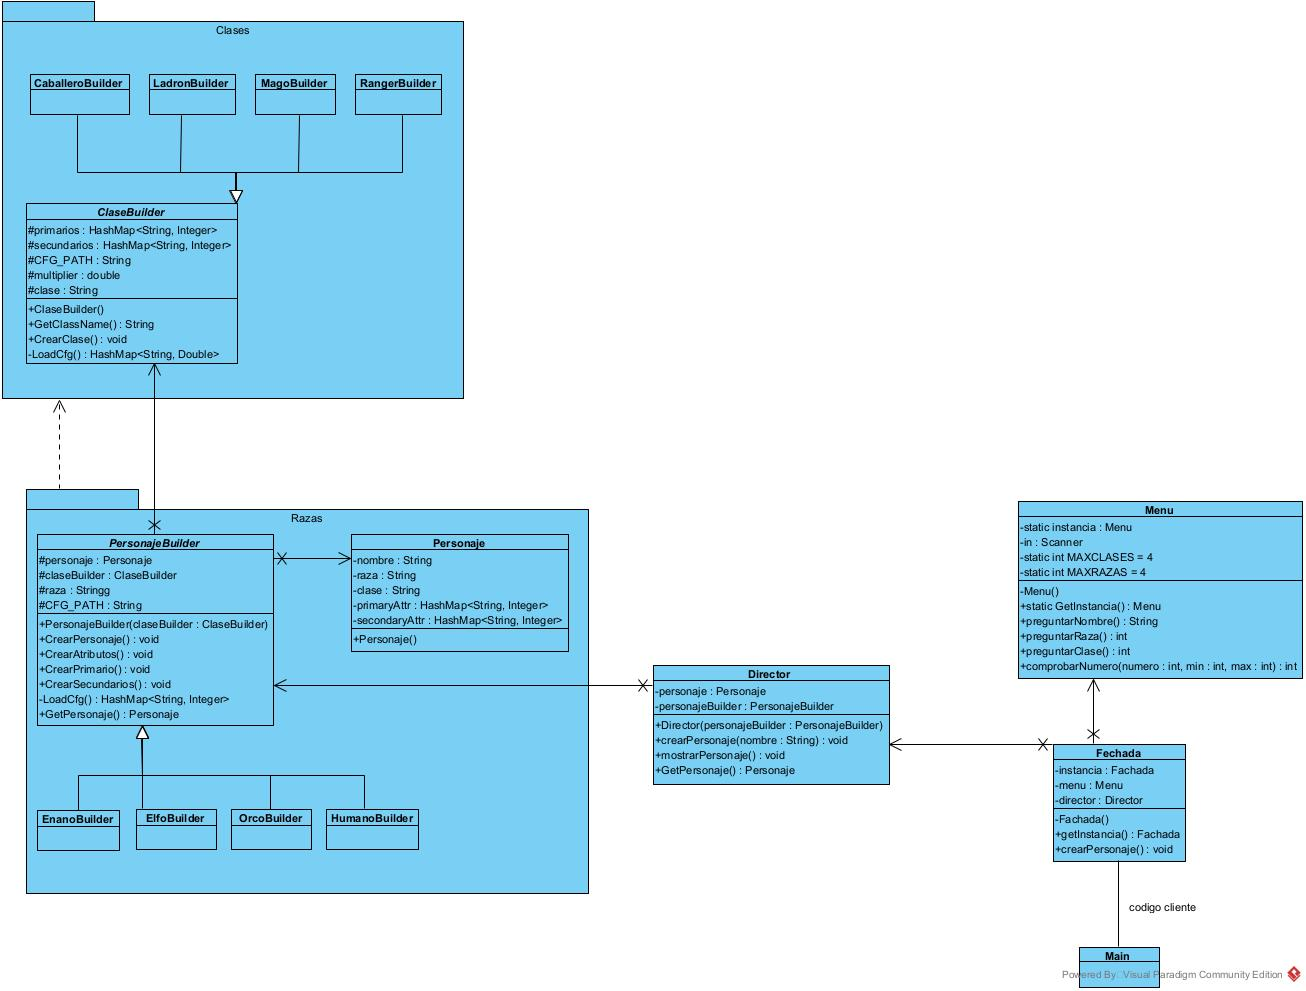
\includegraphics[width=0.6\textwidth]{DS_ej3.jpg}
	\caption{ejercicio 3}
	\label{fig:ej3}
\end{figure}


\subsection{Consideraciones}
Clase ClaseBuilder es una clase abstracta que actua como base para las clases hijas. De modo que hemos optado por dar una funcionalidad 
predeterminada a los métodos para encapsular un comportamiento común y evitar repetir el mismo código en diferentes archivos. De ser necesario una modificación consideramos
que es adecuado que cada clase hija mediante override especialice su comportamiento.

Mismo razonamiento se ha aplicado a PersonajeBuilder

Utilizamos clase Director para abstraer el proceso de creación del personaje, es decir, esta clase se encarga de orquestar los pasos necesarior para construir el objeto de tipo Personaje 

Utilizamos Menu para recoger el input del usuario. Se trata de un Singleton pues pensamos que al interactuar a traves de la terminal no tiene sentido que existan muchos objetos de Menu instaciados  


Por últmo, utilizamos clase Fachada ofrecemos una interfaz unificada para la interacción con el sistema. De esta forma simplificamos el uso de las clases por el código cliente.

Como conslución, hemos obtenido un sistema con bajo nivel de acoplamiento. Cada modulo es responsable de una tarea especifica con su lógica adecuada



\section{Ejercicio 5}
\subsection{Análisis}
En este problema se pide diseñar y realizar una aplicación de WebScraping en Python donde se utilice el Patrón \textit{Strategy} para scrapear información en vivo de acciones.  Para ello se seguirán dos estrategias cada una usando una biblioteca distinta de Python: BeautifulSoup y Selenium.

\subsection{Strategy}
El patrón \textit{Strategy} o \textit{Estrategia} define una familia de algoritmos, encapsula cada uno y los hace intercambiables en tiempo de ejecución. Para ello definimos una clase abstracta llamada \textit{ScraperStrategy} y las estategias de scrapping correspondientes \textit{BeautifulSoupScraper} y \textit{SeleniumScraper}. Además, es necesario crear un clase que sirva para intercambiar las estrategias definidas en cada ejecución, sirviendo para esto la clase \textit{Context}.

\begin{figure}[h]
	\centering
        \vspace{15pt}
	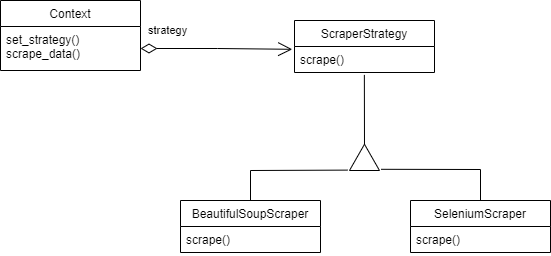
\includegraphics[width=0.6\textwidth]{DS_ej5.drawio.png}
	\caption{Strategy}
	\label{fig:strategy}
\end{figure}


\subsection{Selenium}
Horadando en el código de cada estrategia de scrapping, \textit{SeleniumScraper} ha supuesto un ejercicio de mayor complejidad. Al intentar llevar a cabo este algoritmo, en primera instancia, obteníamos errores debido a la ventana emergente que informa de las cookies nada más entrar en la web. Para sortearla, es necesario pulsar sobre cualquiera de los botones de \textit{Aceptar} o \textit{Rechazar}, sin embargo, estos botones son visibles únicamente si la pantalla cumple unas propiedades específicas de tamaño, si no, es necesario realizar un scroll vertical para alcanzar dichos botones. La solución planteada a esta tesitura ha sido primero maximizar la ventana, garantizando así la visibilidad de los botones, para luego pulsar sobre el botón de \textit{Rechazar} y finalmente acceder a los datos que queremos obtener.



\end{document} 